% $Header$

\documentclass{beamer}

\usepackage[english]{babel}
\usepackage[latin1]{inputenc}
\usepackage{times}
\usepackage{listings}

% https://www.sharelatex.com/learn/Inserting_Images
\usepackage{graphicx}
\graphicspath{ {images/} }

\title{Design Patterns}
\subtitle{aka Object Oriented Programming}

\AtBeginSection{\frame{\sectionpage}}
\AtBeginSubsection{\frame{\subsectionpage}}

\setbeamersize{text margin left=2mm,text margin right=2mm} 

% https://www.sharelatex.com/learn/Paragraph_formatting#/Paragraph_spacing
\renewcommand{\baselinestretch}{1.5}

\lstset{
    % https://tex.stackexchange.com/a/34690/137042
    basicstyle=\fontfamily{pcr}\footnotesize\color{yellow},
    backgroundcolor=\color{black},
    frame=single
}

\begin{document}

\begin{frame}
  \titlepage
\end{frame}

\begin{frame}{Outline}
  \tableofcontents
\end{frame}

\section{Fundamentals}

\begin{frame}{Abstraction}
    \par Delineates a simplified, context-specific representation of a thing.
    \begin{itemize}
        \item Ignores contextually irrelevant details.
        \item Includes contextually relevant details.
    \end{itemize}
\end{frame}

\begin{frame}{Encapsulation}
    \par Restricts outside access to a things parts.
    \par Bundles a things state with the routines that use that state.
\end{frame}

\begin{frame}{Inheritance}
    \par Grants one thing the capabilities of another thing.
    \par Is not the same as though often agrees with subtyping.
    \par Includes prototypal and class-based inheritance.
\end{frame}

\begin{frame}{Polymorphism}
    \par Pluralizes the numbers of types on which a routine can operate.
    \begin{itemize}
        \item Ad hoc / static polymorphism (aka method overloading)
        \item Parameteric polymorphism (aka generics)
        \item Subtype polymorphism
    \end{itemize}
\end{frame}

\section{Principles}

\subsection{A class should have only one reason to change.}

\begin{frame}{What does it mean?}
    \par A reason to change is a responsibility or an axis-of-change.
    \par Change refers to changes in source code not to variables at runtime.
    \par Example responsibilities: print an invoice, calculate tax.
\end{frame}

\begin{frame}{Why does it matter?}
    \begin{itemize}
        \item Clients can consume individual responsibilities.
        \item Responsibilities can change without breaking each other.
        \item Responsibilities can be recompiled independently.
    \end{itemize}
    \par The art is to balance rigidly and needless complexity. 
\end{frame}

\begin{frame}{}
    \lstinputlisting{reason-to-change-01.ts}
\end{frame}

\begin{frame}{}
    \lstinputlisting{reason-to-change-02.ts}
\end{frame}

\subsection{Classes should be open to extension and closed for modification.}

\begin{frame}{What does it mean?}
    \par Change the way a module behaves,
    \par without changing its source code.
    \par How? Use abstraction.
    \par E.g. A draw() method ought to be closed against
    \begin{itemize}
        \item new shapes (via a Shape abstraction),
        \item new ways to order shapes (via an ordering abstraction), though
        \item cannot be closed against all changes. 
    \end{itemize}
\end{frame}

\begin{frame}{Why does it matter?}
    \par Protect existing code against breaking changes.
\end{frame}

\begin{frame}{}
    \lstinputlisting{open-closed-01.ts}
\end{frame}

\begin{frame}{}
    \lstinputlisting{open-closed-02.ts}
\end{frame}

\subsection{Depend on abstractions not on concrete classes.}

% http://aspiringcraftsman.com/2008/12/28/examining-dependency-inversion/

\begin{frame}{What does it mean?}
    \par Also known as the Dependency Inversion Principle.
    \par It inverts the traditional, procedural dependency hierarchy.
    \begin{itemize}
        \item High-level modules should not depend upon low-level modules. Both should depend on abstractions.
        \item Abstractions should not depend upon details. Details should depend upon abstractions.
    \end{itemize}
    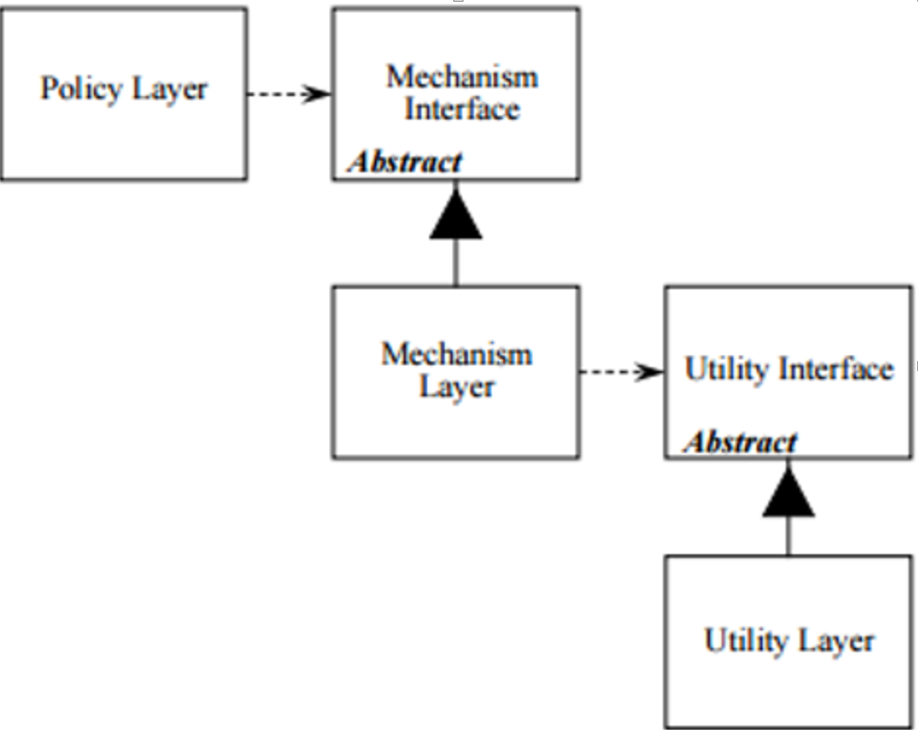
\includegraphics{abstractions-not-concrete-classes-01}
    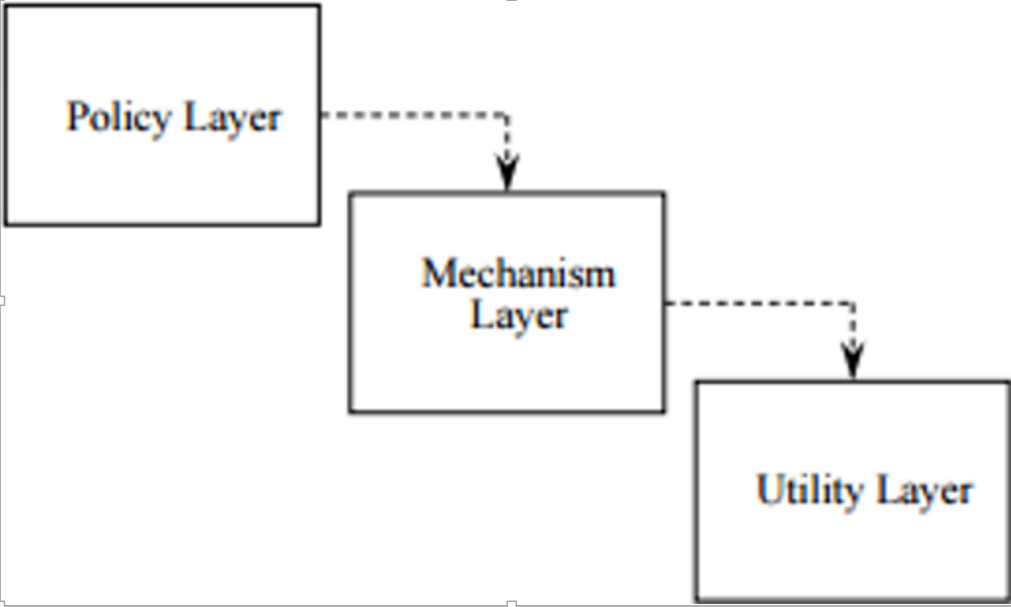
\includegraphics{abstractions-not-concrete-classes-02}
\end{frame}

\begin{frame}{Why does it matter?}
    \par Without inversion, changing the utility layer may effect the policy layer. 
\end{frame}

\begin{frame}{}
    \lstinputlisting{abstractions-not-concrete-classes-01.ts}
\end{frame}

\begin{frame}{}
    \lstinputlisting{abstractions-not-concrete-classes-02.ts}
\end{frame}

\subsection{Don't call us, we'll call you.}

\begin{frame}{What does it mean?}
    \par Inversion of Control: 
    \begin{itemize}
        \item Application code defines a routine (operation/function),
        \item plugs that routine into the framework, and 
        \item the framework controls when to execute it.
    \end{itemize}
    \par Whereas libraries tend to provide normal control, 
    \par in which we call the library code,
    \par frameworks tend to provide inversion of control (IoC),
    \par in which the framework calls us.
\end{frame}

\begin{frame}
Inversion of Control is a key part of what makes a framework different to a library.
Martin Fowler (26 June 2005)
\end{frame}

\begin{frame}{Why does it matter?}
\end{frame}

\begin{frame}{Binding to events:}
    \lstinputlisting{inversion-of-control-01.ts}
\end{frame}

\begin{frame}{Implementing interfaces:}
    \lstinputlisting{inversion-of-control-02.ts}
\end{frame}

\subsection{Encapsulate what varies.}

\begin{frame}{What does it mean?}
    \par "What varies" means source code that might change.
    \par "Encapsulate" means restrict outside access to a things parts.
    \par Therefore: Restrict outside access to source code that might change.
    \par This is a principle of procedural, functional, and OO programming.
\end{frame}

\begin{frame}{What causes change?}
    \begin{itemize}
        \item Changing requirements causes change.
        \item Refactoring causes change. 
        \item Performance improvements cause change. 
        \item Changing business needs cause change. 
        \item Improved understanding of the problem causes change. 
        \item Change in government policies causes change.
    \end{itemize}
\end{frame}

\begin{frame}{Why does it matter?}
    \par Why? We can change code later in as few places as possible.
\end{frame}

\begin{frame}{}
    \lstinputlisting{encapsulate-what-varies-01.ts}
\end{frame}

\begin{frame}{}
    \lstinputlisting{encapsulate-what-varies-02.ts}
\end{frame}

\begin{frame}{}
    \lstinputlisting{encapsulate-what-varies-03.ts}
\end{frame}

\subsection{Favour composition over inheritance.}

\begin{frame}{What does it mean?}
\end{frame}

\begin{frame}{Why does it matter?}
\end{frame}

\subsection{Only talk to your friends.}

% http://www.ccs.neu.edu/home/lieber/LoD.html

\begin{frame}{What does it mean?}
    \begin{itemize}
        \item Law of Demeter (1987)
        \item Principle of Least Knowledge
        \item "Only use one dot"
        \item Promotes loose coupling
    \end{itemize}
\end{frame}

\begin{frame}{Why does it matter?}
\end{frame}

\begin{frame}{}
    \lstinputlisting{only-talk-to-friends-01.ts}
\end{frame}

\begin{frame}{}
    \lstinputlisting{only-talk-to-friends-02.ts}
\end{frame}

\subsection{Program to interfaces not to implementations.}

\begin{frame}{What does it mean?}
    \begin{itemize}
        \item Program against a contract, 
        \item which can have many varying implementations.
    \end{itemize}
    \par It is much more general than the dependency inversion principle, which requires:
    \begin{itemize}
        \item that the high-level component owns the interface, and
        \item that object creation happens outside the dependent class.
    \end{itemize}
\end{frame}

\begin{frame}{Why does it matter?}
\end{frame}

\begin{frame}{}
    \lstinputlisting{program-to-interfaces-01.ts}
\end{frame}

\begin{frame}{}
    \lstinputlisting{program-to-interfaces-02.ts}
\end{frame}

\subsection{Strive for loosely coupled designs among objects that interact.}

\begin{frame}{What does it mean?}
\end{frame}

\begin{frame}{Why does it matter?}
\end{frame}

\end{document}

